\documentclass[12pt,letterpaper]{article}
\usepackage{fullpage, lastpage, enumerate, fancyhdr}
\usepackage[top=2cm, bottom=4.5cm, left=2.5cm, right=2.5cm]{geometry}
\usepackage{amsmath,amsthm,amsfonts,amssymb,amscd}
\usepackage{mathrsfs, xcolor, graphicx, subcaption, siunitx}
\usepackage{hyperref}
\graphicspath{{./images}}

\hypersetup{%
  colorlinks=true,
  linkcolor=blue,
  linkbordercolor={0 0 1}
}

\setlength{\parindent}{0.0in}
\setlength{\parskip}{0.05in}

\pagestyle{fancyplain}
\headheight 15pt
\fancyhf[FL]{Matthew Bernstein}
\fancyhf[HR]{\today}
\fancyhf[HL]{ISyE 7406 - Homework 1}
\fancyhf[FC]{}
\fancyhf[FR]{\thepage}
\headsep 1.5em

\title{ISYE 7406 - Homework 1}
\author{Matthew Bernstein}

\begin{document}
\fancypagestyle{plain}{
    \fancyhf{}
    \renewcommand{\headrulewidth}{0pt}
    \renewcommand{\footrulewidth}{0pt}
}
\maketitle
\section*{Introduction}

The purpose of this assignment is to compare two different methods of supervised learning: Linear Regressions and K Nearest Neighboor classifiers. To do so, we used the \textit{zipcode} dataset. This dataset is used for handwriting analysis by representing a 16x16 pixel image of a digit (1-9) as 256 individual greyscale values. We were particularly focused on the digits 2 and 7.

The problem being evaluated is the performance of the 2 different model types, as well as understanding how to properly tune a KNN classifier and the importance and effect of cross validation on model selection.

\section*{Exploratory Data Analysis}

The dataset, after filtering for only the digits 2 and 7, contains 1376 observations. Each observation contains the intended digit, which is the response value, as well as 256 columns describing the greyscale value of each pixel in the 16x16 image. Figure \ref{fig:example} shows an example image representation of one of the observations. Of the 1376 observations, 731, or 53\% of them are for the digit ``2".

\begin{figure}[h]
  \centering
  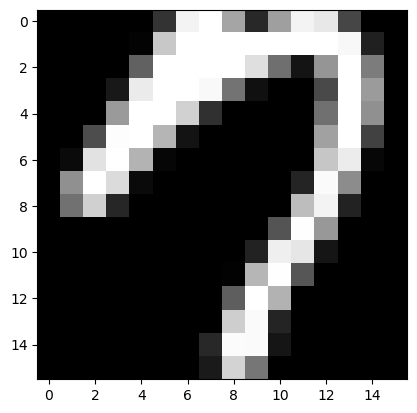
\includegraphics[width=0.2\textwidth]{example}
  \caption{Example image reconstructed from data. Y = 7}
  \label{fig:example}
\end{figure}

Each greyscale value is a number between -1, meaning black, and 1, meaning white. Figure \ref{fig:heatmap} shows a correlation heatmap between each of the pixels as well as the response digit. It does appear that any single pixel has a strong correlation, white for positive and black for negative, with the response variable. Each does appear to be positively correlated with the pixels next to it as well as above and below it. There seems to be some highly negative correlation between the first 2 rows of pixels and pixels towards the last few rows. 

\begin{figure}[h]
  \centering
  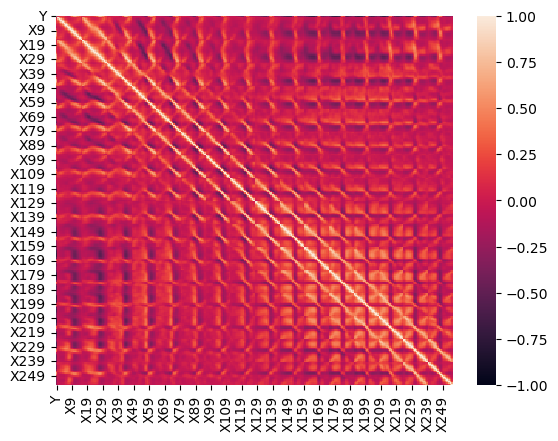
\includegraphics[width=0.7\textwidth]{heatmap}
  \caption{Correlation heatmap between all data columns}
  \label{fig:heatmap}
\end{figure}

When looking at the average response for each image type in Figure \ref{fig:avg_image} shows that a classifier should be fairly accurate given the different images. The average 7 closely resembles a 7 and while the average 2 is less clear, there are distinct regions that separate it from the average 7. Notably, the bottom left and right corners appear light on a 2, but dark in a 7.

\begin{figure}[h]
  \centering
  \begin{subfigure}{0.3\textwidth}
    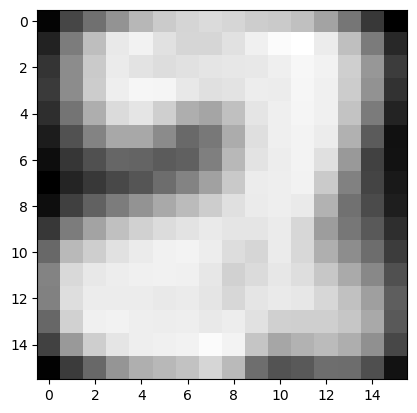
\includegraphics[width=\textwidth]{avg_img}
    \caption{Average of all observations}
  \end{subfigure}
  \begin{subfigure}{0.3\textwidth}
    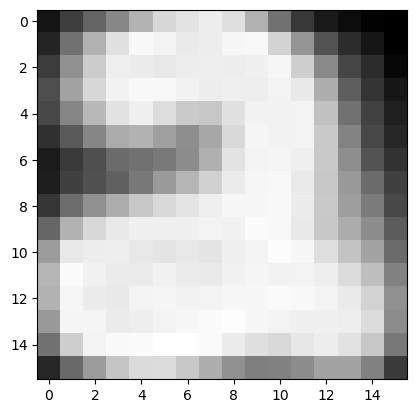
\includegraphics[width=\textwidth]{avg_2}
    \caption{Average ``2''}
  \end{subfigure}
  \begin{subfigure}{0.3\textwidth}
    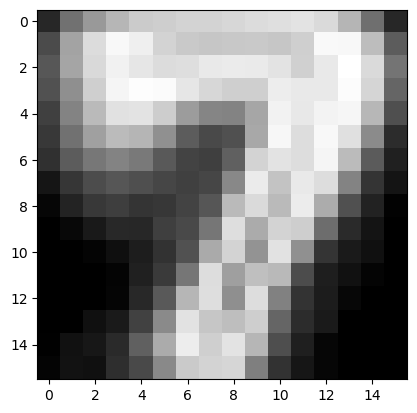
\includegraphics[width=\textwidth]{avg_7}
    \caption{Average ``7''}
  \end{subfigure}
  \caption{Average images for each response type}
  \label{fig:avg_image}
\end{figure}

\section*{Methodology}

Two different models were used in this analysis. First a linear regression model was constructed based on the data. The resulting value was determined to be a ``2'' or a ``7'' depending on if the output of the model was above or below 4.5, the center point between 2 and 7. The 8 KNN classifiers were trained using $k = {1, 3, 5, 7, 9, 11, 13, 15}$. 

Training error was reported for each of the 9 models. They were then tested against the test data set, which had also been filtered for only ``2'' and ``7''. The test error for each model was then calculated. 

Finally, a Monte Carlo cross validation was performed for each of the 9 models. In this, the training and test data sets were combined and then re-split in the same proportions. Each of the 9 models were trained on the new training set and test error was recorded for the new test set. This procedure was performed 100 times and then average test error for each model was calculated. 

\section*{Results}

\begin{table}[h]
  \centering
  \begin{tabular}{|l|c|c|}
    \hline
    Model & Training Error (\%) & Test Error (\%) \\ \hline \hline
    Linear Regression & 0.073 & 1.739 \\ \hline
    KNN, k = 1 & 0.000 & 1.739 \\ \hline
    KNN, k = 3 & 1.017 & 1.449 \\ \hline
    KNN, k = 5 & 1.236 & 1.449 \\ \hline
    KNN, k = 7 & 1.454 & 1.739 \\ \hline
    KNN, k = 9 & 1.599 & 1.739 \\ \hline
    KNN, k = 11 & 1.599 & 1.739 \\ \hline
    KNN, k = 13 & 1.744 & 2.029 \\ \hline
    KNN, k = 15 & 1.744 & 2.029 \\ \hline
  \end{tabular}
  \caption{Training and test errors for all models}
  \label{tab:results}
\end{table}

Table \ref{tab:results} shows the training and test error results from the 9 tested models. Each model shows training error lower than test error, which is expected, however, they are quite close meaning each of the models is fairly robust. Going by test error, the $k = 3$ and $k = 5$ models performed the best with the linear regression and $k = {1, 7, 9, 11}$ performing slighly worse.

Higher orders of $k$ can cause problems on the borders of the data as the farther out data could swing the internal ``vote'' towards a different classification. This is demonstrated by the data since the lower values of $k$ out perform larger values. 

Table \ref{tab:cv} shows the Monte Carlo Cross Validation results. On a whole, error and variance are low for all methods. Linear Regression performs the best over all the different models as it has the lowest average error and the second lowest error variance. Suprisingly, KNN $k=1$ performs the best of all KNN models. Error and variance geenrally rise as $k$ increases with a large jump in average error at $k=5$ and a large jump in error variance at $k=7$. 

\begin{table}[h]
  \centering
  \begin{tabular}{|l|c|c|}
    \hline
    Model & CV Test Error (\%) & CV Test Variance \\ \hline \hline
    Linear Regression & 1.176 & \num{2.6e-5} \\ \hline
    KNN, k = 1 & 1.258 & \num{2.5e-5} \\ \hline
    KNN, k = 3 & 1.310 & \num{2.8e-5} \\ \hline
    KNN, k = 5 & 1.528 & \num{4.0e-5} \\ \hline
    KNN, k = 7 & 1.673 & \num{4.5e-5} \\ \hline
    KNN, k = 9 & 1.742 & \num{4.8e-5} \\ \hline
    KNN, k = 11 & 1.855 & \num{5.2e-5} \\ \hline
    KNN, k = 13 & 1.947 & \num{5.1e-5} \\ \hline
    KNN, k = 15 & 1.986 & \num{5.6e-5} \\ \hline
  \end{tabular}
  \caption{Training and test errors for all models}
  \label{tab:cv}
\end{table}

Based on the results from the test set and cross validation, a KNN classifier with $k=3$, would be the recommended model moving forward. 

\section*{Conclusion}

In conclusion, both Linear Regression models and KNN classifiers can perform quite well for performing classification tasks. Even though Linear Regression tends to be less accurate for discrete data, it peformed exceedingly well for this dataset. It would be interesting to see if it maintains its peformance accross the whole data set, and not just a filtered subsection. 

For the KNN classifiers, it was shown that higher orders of $k$ can have a lot more variance accross cross validation trials and can be less accurate. Therefore, it is recommended to keep the $k$ parameter low to ensure that only the most relevant neighbors are considered when classifying new data. 

\end{document}